\section{TO-BE} \label{sec:tobe}
\subsection{Main model}

\begin{figure}[H]
    \centering
    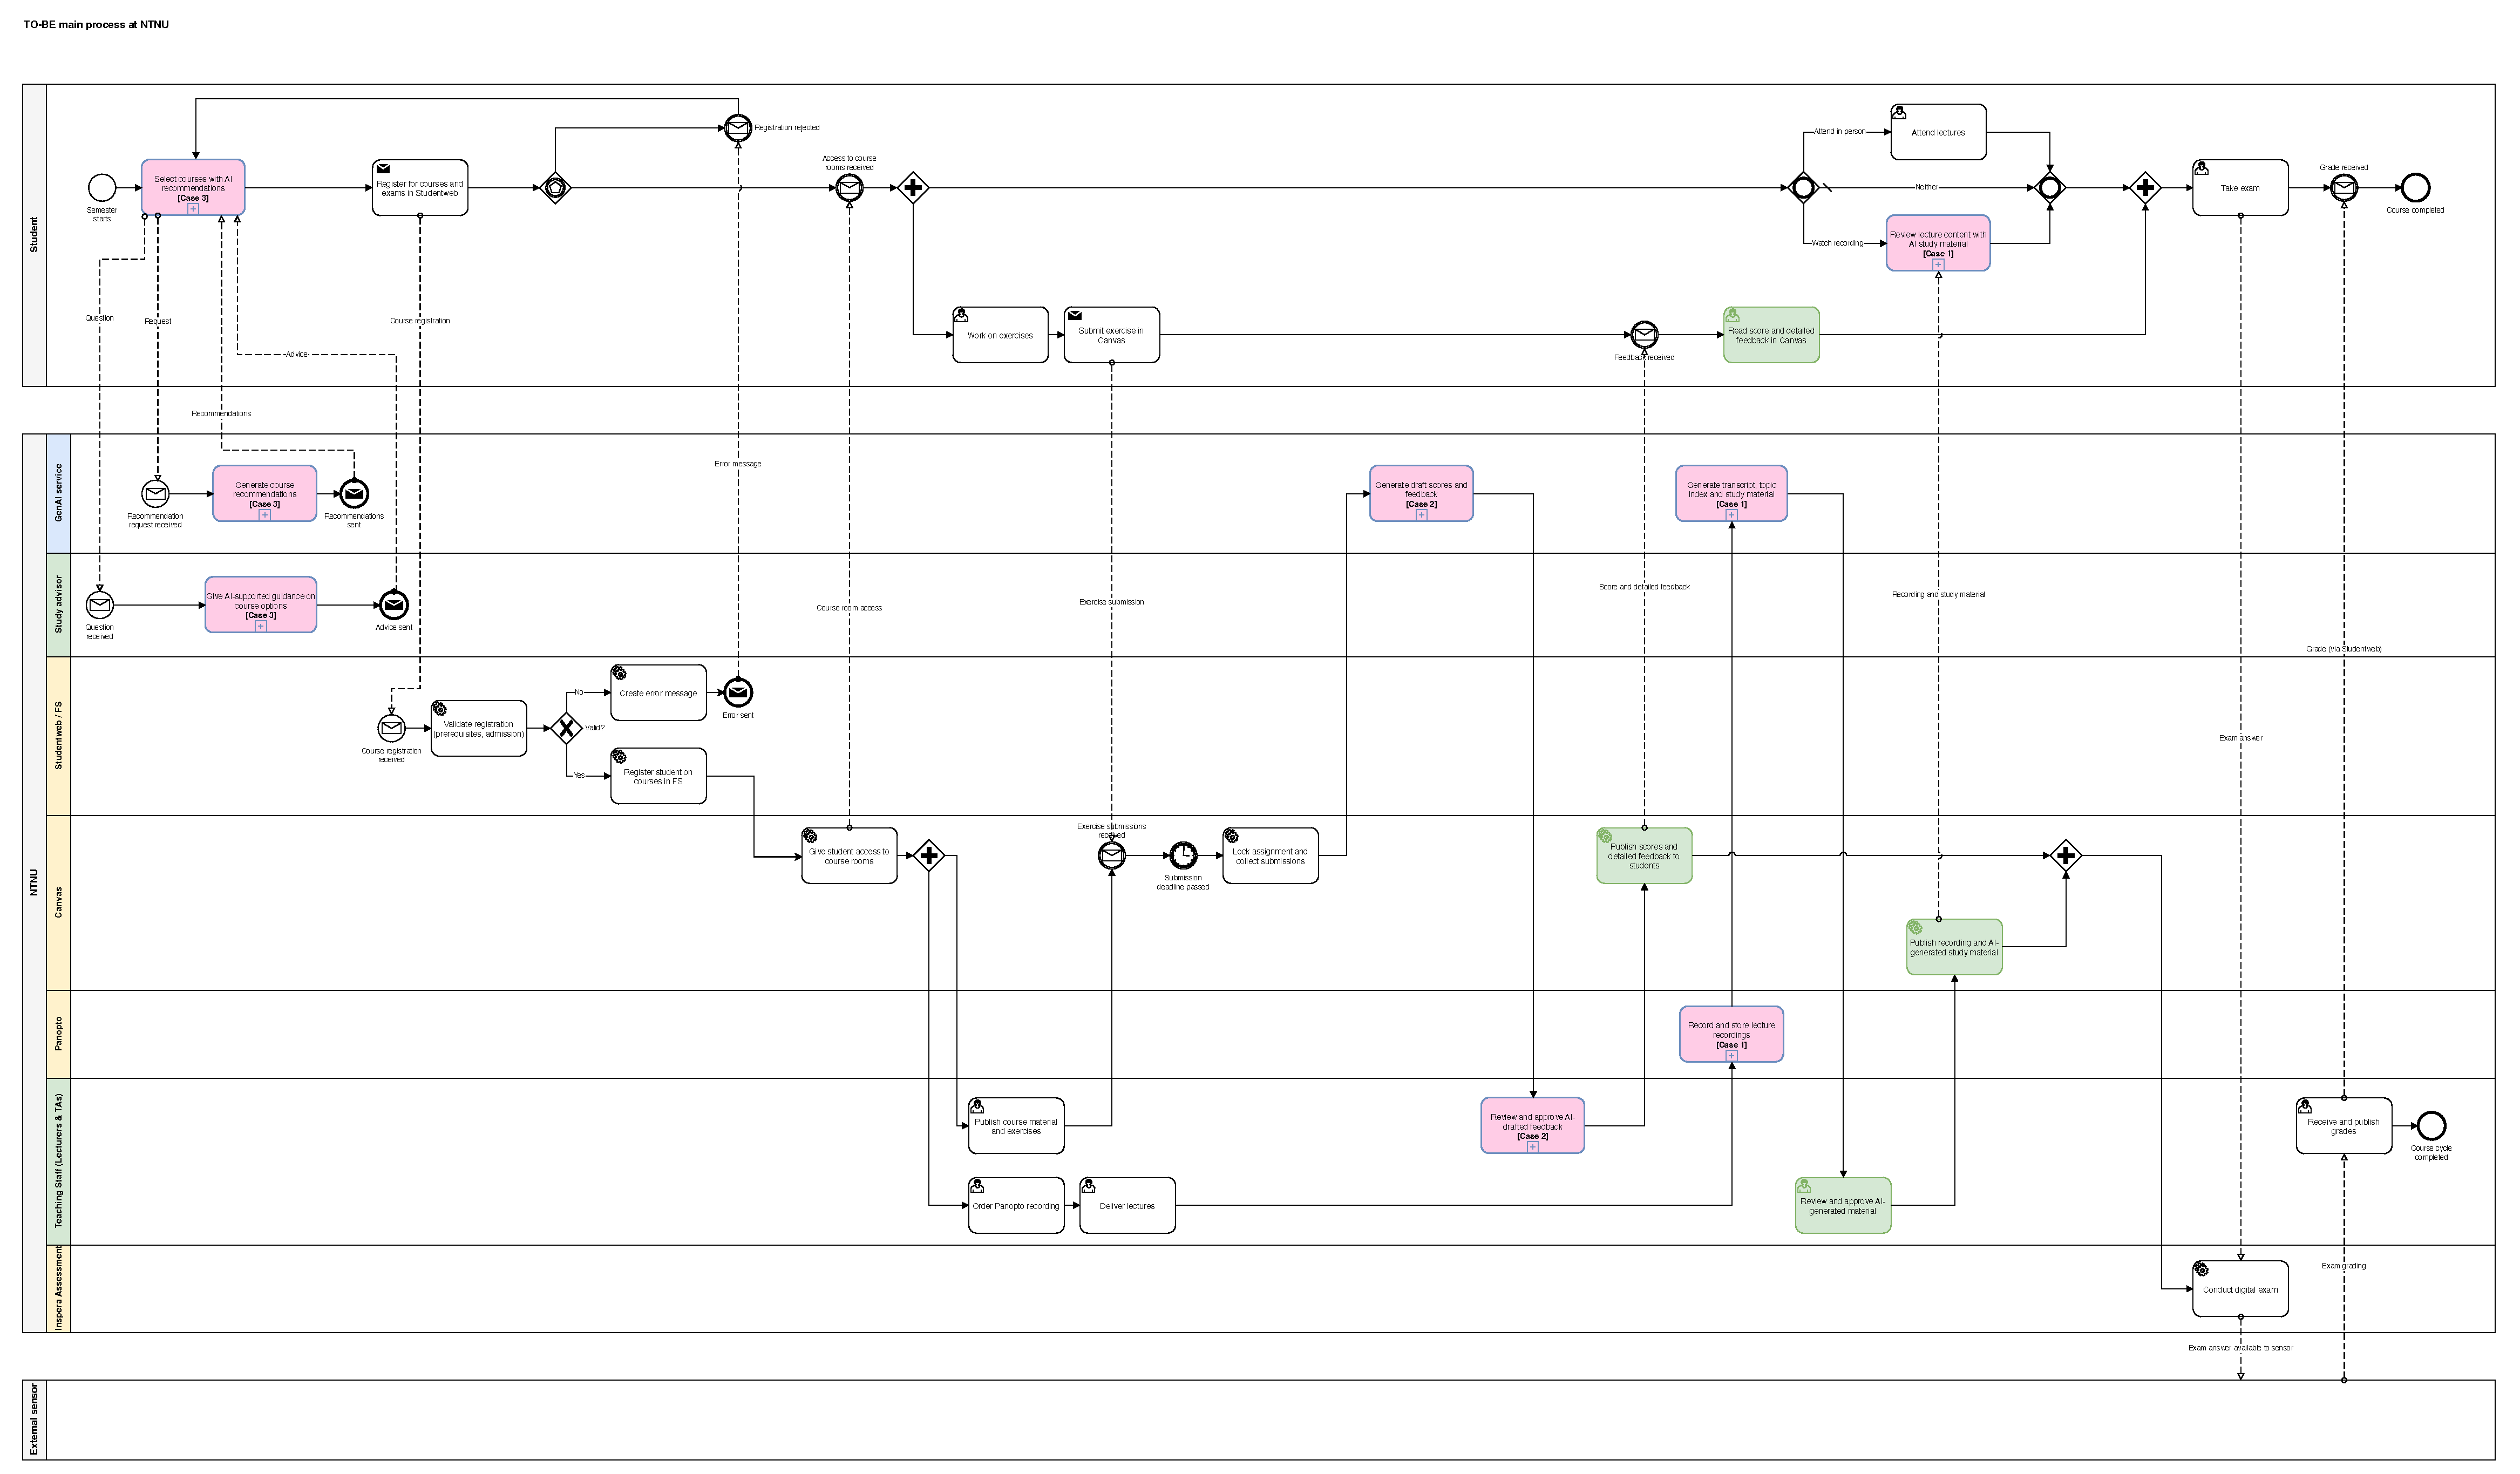
\includegraphics[width=\textwidth]{Images/main_to-be.drawio.pdf}
    \caption{TO-BE main process at NTNU}
    \label{fig:main_to-be}
\end{figure}



Figure~\ref{fig:main_to-be} presents a high-level BPMN model of the proposed learning process at NTNU. To make it easy to compare with the AS-IS model (Figure~\ref{fig:main_as-is}), the model keeps the same structure. It has the same three pools, \textit{Student}, \textit{NTNU} and \textit{External sensor}, and the same lanes for Study advisor, Studentweb/FS, Canvas, Panopto, Teaching Staff (lecturers and teaching assistants) and Inspera Assessment. The only new lane is \textit{GenAI service}. It is placed in the NTNU pool and is shared by all three cases. NTNU is responsible for the this service, since it is integrated with NTNU's existing systems, and the student does not interact with it as a separate party. As in the AS-IS model, human actors are shown in green lanes and information systems in yellow lanes. Collapsed sub-processes are marked pink and are explained in the following sections. Tasks that are new or changed compared to the AS-IS model are marked green.

\textbf{Course selection and registration:} The process starts at the beginning of the semester, when the student selects courses. This is now modelled as the collapsed sub-process \textit{Select courses with AI recommendations} (Case 3) in the Student pool. Instead of researching the options manually, the student sends a request with their interests and goals to the GenAI service lane. There, the message start event \textit{Recommendation request received} starts the collapsed sub-process \textit{Generate course recommendations} (Case 3), and a ranked shortlist of courses is sent back to the student. If the student still needs advice, a question is sent to the Study advisor lane. The study advisor now answers in the collapsed sub-process \textit{Give AI-supported guidance on course options} (Case 3) and sends the advice back to the student. The registration itself is unchanged from the AS-IS model. The student registers for courses and exams in Studentweb, and the registration is validated against the prerequisites and admission rules in the Studentweb/FS lane. On the student side, an event-based gateway waits for either an error message or access to the course rooms in Canvas.

\textbf{The learning phase:} The learning phase is still modelled as two parallel tracks, one for lectures and one for exercises. In the lecture track, the teaching staff order a Panopto recording and deliver the lectures. The lectures are recorded and stored by Panopto in the collapsed sub-process \textit{Record and store lecture recordings} (Case 1), which is unchanged from the AS-IS model. The stored recording is then passed to the GenAI service, which produces a transcript, a topic index and study material in the collapsed sub-process \textit{Generate transcript, topic index and study material} (Case 1). Before anything is published, the teaching staff perform the new task \textit{Review and approve AI-generated material}. Canvas then publishes the recording together with the approved material in \textit{Publish recording and AI-generated study material}. On the student side, the inclusive gateway is unchanged. The student may attend the lecture in person, watch the recording, or do both, and the default flow \textit{Neither} still allows the student to skip the lecture track. The student's review of the lecture is now modelled as the collapsed sub-process \textit{Review lecture content with AI-generated study material} (Case 1).

In the exercise track, the teaching staff publish course material and exercises. The student works on the exercises and submits them in Canvas. When the submission deadline has passed, Canvas locks the assignment and collects the submissions. Unlike in the AS-IS model, the submissions are not distributed directly among the TAs. They are first sent to the GenAI service, which drafts a score and detailed feedback for each submission in the collapsed sub-process \textit{Generate draft scores and feedback} (Case 2). The teaching staff then review, adjust and approve the drafts in the collapsed sub-process \textit{Review and approve AI-drafted feedback} (Case 2), which replaces \textit{Assess exercises and give feedback} from the AS-IS model. Canvas publishes the approved scores and detailed feedback to the students, and the student reads them in the changed task \textit{Read score and detailed feedback in Canvas}. As in the AS-IS model, the exercises are mandatory and must be approved before the student can take the exam. The parallel gateway that joins the two tracks before the exam is therefore kept.

\textbf{Exam and grading:} The exam and grading part of the process is unchanged. A parallel gateway in the Canvas lane ensures that both the publishing of recordings and study material and the publishing of feedback are completed before the digital exam is conducted in Inspera Assessment. The exam answers are made available to the external sensor, who grades the exam and returns the result to NTNU. The teaching staff receive and publish the grades, and the student is notified of the final grade through Studentweb. The GenAI service is deliberately not used in the exam or in the final grading.

Compared with the AS-IS model, the TO-BE model shows that GenAI is added between the existing systems rather than replacing them. Studentweb, FS, Canvas, Panopto and Inspera keep the same roles as before. In all three cases, a human actor is placed between the GenAI service and the student. Lecturers approve the study material, TAs approve scores and feedback, study advisors review the AI suggestions, and the student makes the final choice of courses. This human-in-the-loop design is important, since output from GenAI can sound convincing but still be wrong \parencite{qian2025}. The solution is therefore a process innovation within existing systems, closer to sustaining innovation and continuous improvement than to re-engineering the whole teaching process. The GenAI service supports decisions and knowledge work, while its still people making the decisions.

\subsection{Case 1} \label{subsec: tobeCase1}

% 4. Teaching at NTNU Next-GenAI: the TO-BE situation – Describe the TO-BE situation by
% detailing how the sub-processes the group focuses on will change due to the new or changed
% use of Generative AI technology. New or changed functionality must be properly described.
% 3
% Also, it should be indicated by new BPMN models how the sub-processes change. (approx. 6
% pages, including the models). Include in the models a sustainability analysis using the SUSAF
% framework as presented in the lectures by John Krogstie.

% ####################################### utkast

\begin{figure}[htbp]
    \centering
    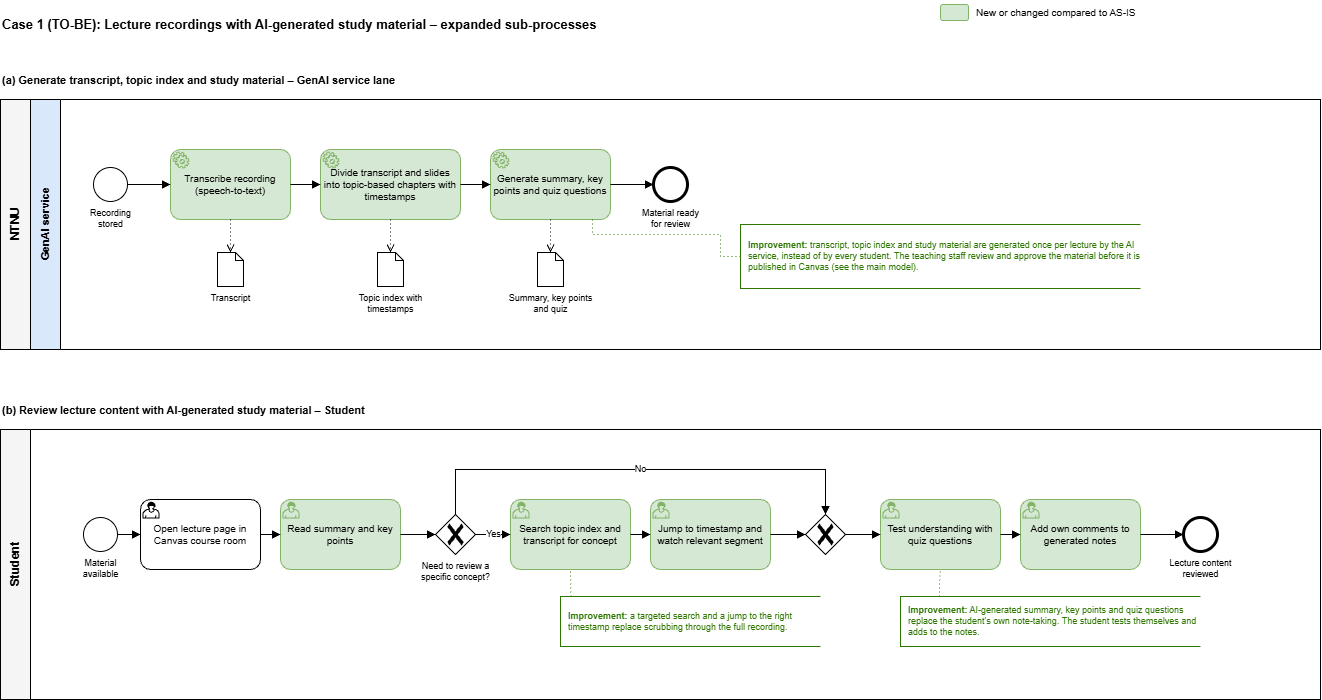
\includegraphics[width=\textwidth]{Images/case1/case1_to-be.drawio.png}
    \caption{Case 1 TO-BE BPMN models: (a) Generate transcript, topic index and study material, (b) Review lecture content with AI study material}
    \label{fig:case1-tobe}
\end{figure}

This section describes the TO-BE model for Case 1, ``Lecture content is not searchable or reusable''. As described in the AS-IS analysis (Figure~\ref{fig:case1}), the process has three main pain points. First, Panopto only stores the raw video, and nothing processes the content of the recording. There is no transcript, topic-based index, summary or study material, and the only navigation aid is a table of contents based on slide titles. Second, the student therefore has to scrub through the video to find a specific concept. Third, every student repeats the same work of reviewing the lecture and making notes, for every lecture. The TO-BE model in Figure~\ref{fig:case1-tobe} addresses these pain points by letting a GenAI service generate a transcript, a topic index and study material from each recording (Figure~\ref{fig:case1-tobe}a), which the student then uses to review the lecture (Figure~\ref{fig:case1-tobe}b).

\paragraph{Model overview}
In the TO-BE main model (Figure~\ref{fig:main_to-be}), Case 1 is represented by three collapsed subprocesses, each placed in the lane of the actor that performs it: \textit{Record and store lecture recordings} in the Panopto lane, which is unchanged from the AS-IS model, \textit{Generate transcript, topic index and study material} in the new GenAI service lane, and \textit{Review lecture content with AI-generated study material} in the Student pool. The activities performed by the teaching staff and Canvas, reviewing and approving the generated material and publishing it in the course room, are shown in the main model. Figure~\ref{fig:case1-tobe} expands the two new subprocesses. Activities that are new or changed compared to the AS-IS model are marked green, and the improvements are described in green annotations.

\paragraph{Subprocess (a): Generate transcript, topic index and study material}
In the AS-IS model, the process ended when the recording was stored in the Panopto database, and the raw video was made available to the students. In the TO-BE model, the stored recording is first sent to the GenAI service. The subprocess starts with \textit{Recording stored} and consists of three service tasks. First, the recording is transcribed using speech-to-text, which produces a \textit{Transcript}. Second, the transcript and the lecture slides are divided into topic-based chapters with timestamps. This produces a \textit{Topic index with timestamps}, which replaces the table of contents based on slide titles. Third, the GenAI service generates a summary, key points and quiz questions from the content of the lecture. The subprocess ends with \textit{Material ready for review}. Since all tasks are automated, the material is produced once per lecture, instead of once per student as in the AS-IS process. %TODO Skrive om improvements her?

\paragraph{Subprocess (b): Review lecture content with AI-generated study material}
The subprocess starts when the material is available in Canvas, and the student opens the lecture page in the Canvas course room. Instead of starting with the full video, the student first reads the summary and key points to get an overview of the lecture. An exclusive gateway, \textit{Need to review a specific concept?}, then decides the next step. If the answer is yes, the student searches the topic index and transcript for the concept and jumps directly to the timestamp of the relevant segment and watches it. If the answer is no, the student continues directly. The two paths merge, and the student tests their understanding with the generated quiz questions. Finally, the student adds their own comments to the generated notes, and the subprocess ends with \textit{Lecture content reviewed}. %TODO skrive om forbedringer her?

Compared with the AS-IS model (Figure~\ref{fig:case1}), the two activities that were marked as pain points are replaced with activities that improves the effectiveness of the process. The looping task \textit{Scrub through full recording to find concept} is replaced by a targeted search followed by a jump to the right timestamp. The manual task \textit{Write own notes and study material} is replaced by AI-generated material that the student reads, tests themselves on and adds to. The student is still actively engaged with the content, but their time is spent on understanding the lecture rather than on finding the relevant segments and writing notes from scratch.

\paragraph{Changes in the main model}
In the TO-BE main model (Figure~\ref{fig:main_to-be}), the generated material is sent to the teaching staff, who review and approve it before anything is published. This is a new manual control step. It ensures that the lecturer stays responsible for the course content, and that errors from the GenAI service, such as incorrect terminology or misinterpreted content, are caught before they reach the students. Keeping a human in the loop is important, since output from GenAI can sound convincing, but still be wrong (Qian 2025). After the lecturer approves the AI-generated material, Canvas publishes the recording together with the transcript, topic index and study material in the course room, and the students are notified. The workload of making the lecture content usable is thereby moved from each individual student to an automated service, with the teaching staff responsible for quality assurance. %TODO Skrive noe om mer workload på foreleser?






\subsection{Case 2} \label{subsec: tobeCase2}

\begin{figure}[H]
    \centering
    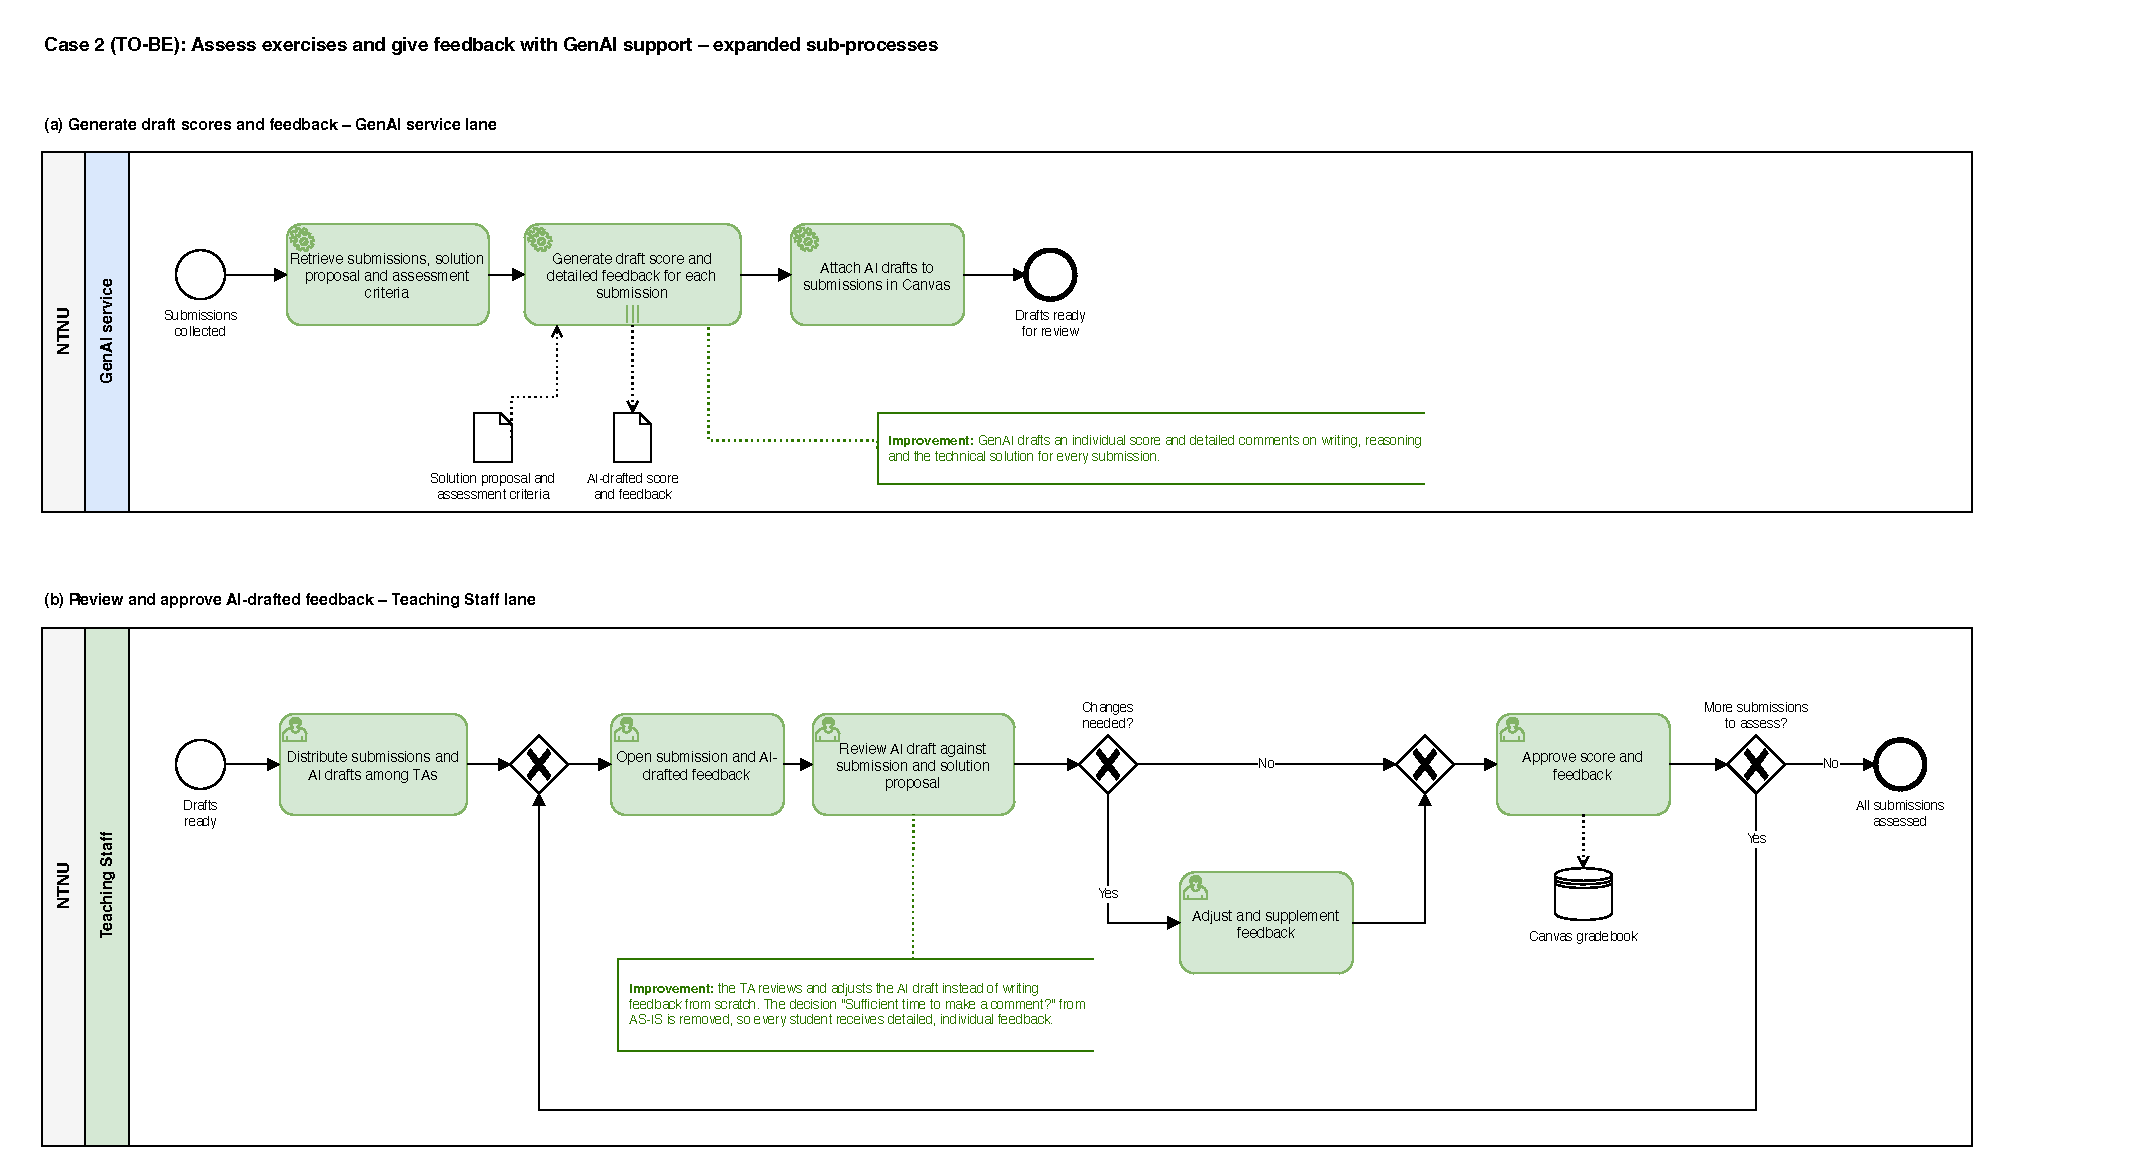
\includegraphics[width=\textwidth]{Images/case2/case2_to-be.drawio.pdf}
    \caption{Case 2 TO-BE BPMN model}
    \label{fig:case2tobe}
\end{figure}

This section describes the TO-BE model for Case 2 "Feedback on exercises and assignments is minimal".  %TODO Er dette riktig navn? Stemmer ikke med det som står i TO-BE-modellen

As described in Section 3.2.2, the AS-IS process for giving feedback on exercises has three main pain points, which are marked in Figure~\ref{fig:case2}. First, every submission is opened, checked and scored manually by a teaching assistant (TA), so the workload grows with the size of the cohort. Second, whether a written comment is given at all depends on the time available to the TA, not on the needs of the student. Third, when a comment is written, it is often short and generic. The problem is not that the TAs put too little effort into giving feedback, but that they have so many submissions to assess that there is little time left for each student. As a result, students receive little actionable guidance on how to improve their writing, reasoning or technical solutions. The TO-BE model in Figure~\ref{fig:case2tobe} addresses these pain points by letting a GenAI service draft a score and detailed feedback for every submission (Figure~\ref{fig:case2tobe}a), so that the TAs review and adjust the drafts instead of writing the feedback from scratch (Figure~\ref{fig:case2tobe}b).

\paragraph{Model overview} 
In the TO-BE main model (Figure~\ref{fig:main_to-be}), Case 2 is represented by two collapsed subprocesses, each placed in the lane of the actor that performs it: \textit{Generate draft scores and feedback} in the new GenAI service lane, and \textit{Review and approve AI-drafted feedback} in the Teaching Staff lane. The Canvas activities around them are shown in the main model. Canvas locks the assignment and collects the submissions when the deadline has passed, and publishes the scores and feedback to the students when all submissions have been reviewed. Figure~\ref{fig:case2tobe} expands both subprocesses. Activities that are new or changed compared to the AS-IS model are marked green, and the improvements are described in green annotations.

\paragraph{Subprocess (a): Generate draft scores and feedback} 
In the AS-IS model, the submissions were distributed among the TAs as soon as they had been collected. In the TO-BE model, they are first sent to the GenAI service. The subprocess consists of three service tasks. First, the service retrieves the submissions together with the solution proposal and the assessment criteria for the exercise. Second, it generates a draft score and detailed feedback for each submission, commenting on the student's writing, reasoning and technical solution. The draft score is based on the student's work compared to the solution proposal and the assessment criteria. This task is modeled as a parallel multi-instance task, since it is performed once for every submission and the submissions can be processed at the same time. The result is the data object \textit{AI-drafted score and feedback}. Third, the drafts are attached to the submissions in Canvas, and the subprocess ends with \textit{Drafts ready for review}. Since every draft is based on the same criteria, the feedback should also be more consistent across TAs.

\paragraph{Subprocess (b): Review and approve AI-drafted feedback} When the drafts are ready, the submissions and drafts are distributed among the TAs, as shown in Figure~\ref{fig:case2tobe}b. As in the AS-IS model, the assessment is modeled as a loop that is repeated for each submission. The TA opens the submission together with the AI-drafted feedback, and reviews the draft against the submission and the solution proposal. The purpose of this step is to make sure that the draft does not contain anything incorrect, for example a correct but unconventional solution being marked as an error. Keeping a human in the loop is important, since output from GenAI can sound convincing but still be wrong (Qian 2025). An exclusive gateway, \textit{Changes needed?}, then decides the next step. If the draft needs changes, the TA adjusts and supplements the feedback. If not, the draft is used as it is. The two paths merge, and the TA approves the score and feedback, which is stored in the Canvas gradebook. A second gateway checks whether there are more submissions to assess, and the loop is repeated until all submissions have been reviewed.

Compared with the AS-IS model (Figure~\ref{fig:case2}), the TA no longer writes the feedback from scratch, and the gateway \textit{Sufficient time to make a comment?} is removed. Written feedback is therefore no longer skipped when time is short, but given to every student. The TA is still responsible for the assessment, but the work moves from producing feedback to quality-assuring it. The decision the TA has to make is no longer whether there is time to give feedback at all, but whether the AI draft needs changes.

\paragraph{Changes in the main model} In the TO-BE main model (Figure~\ref{fig:main_to-be}), Canvas publishes the approved scores and detailed feedback to the students, and the student task \textit{Read score and comment in Canvas} is replaced by \textit{Read score and detailed feedback in Canvas}. Instead of receiving only a score or a short comment, every student now receives detailed, individual feedback on what was done well and what can be improved. The goal is that students can take this feedback with them into their further work, which supports the case description's goal of ``assisting the development of students' writing skills and critical thinking/reflecting skills''.

\subsection{Case 3} \label{subsec: tobeCase3}

\begin{figure}[H]
    \centering
    \begin{subfigure}{\textwidth}
        \centering
        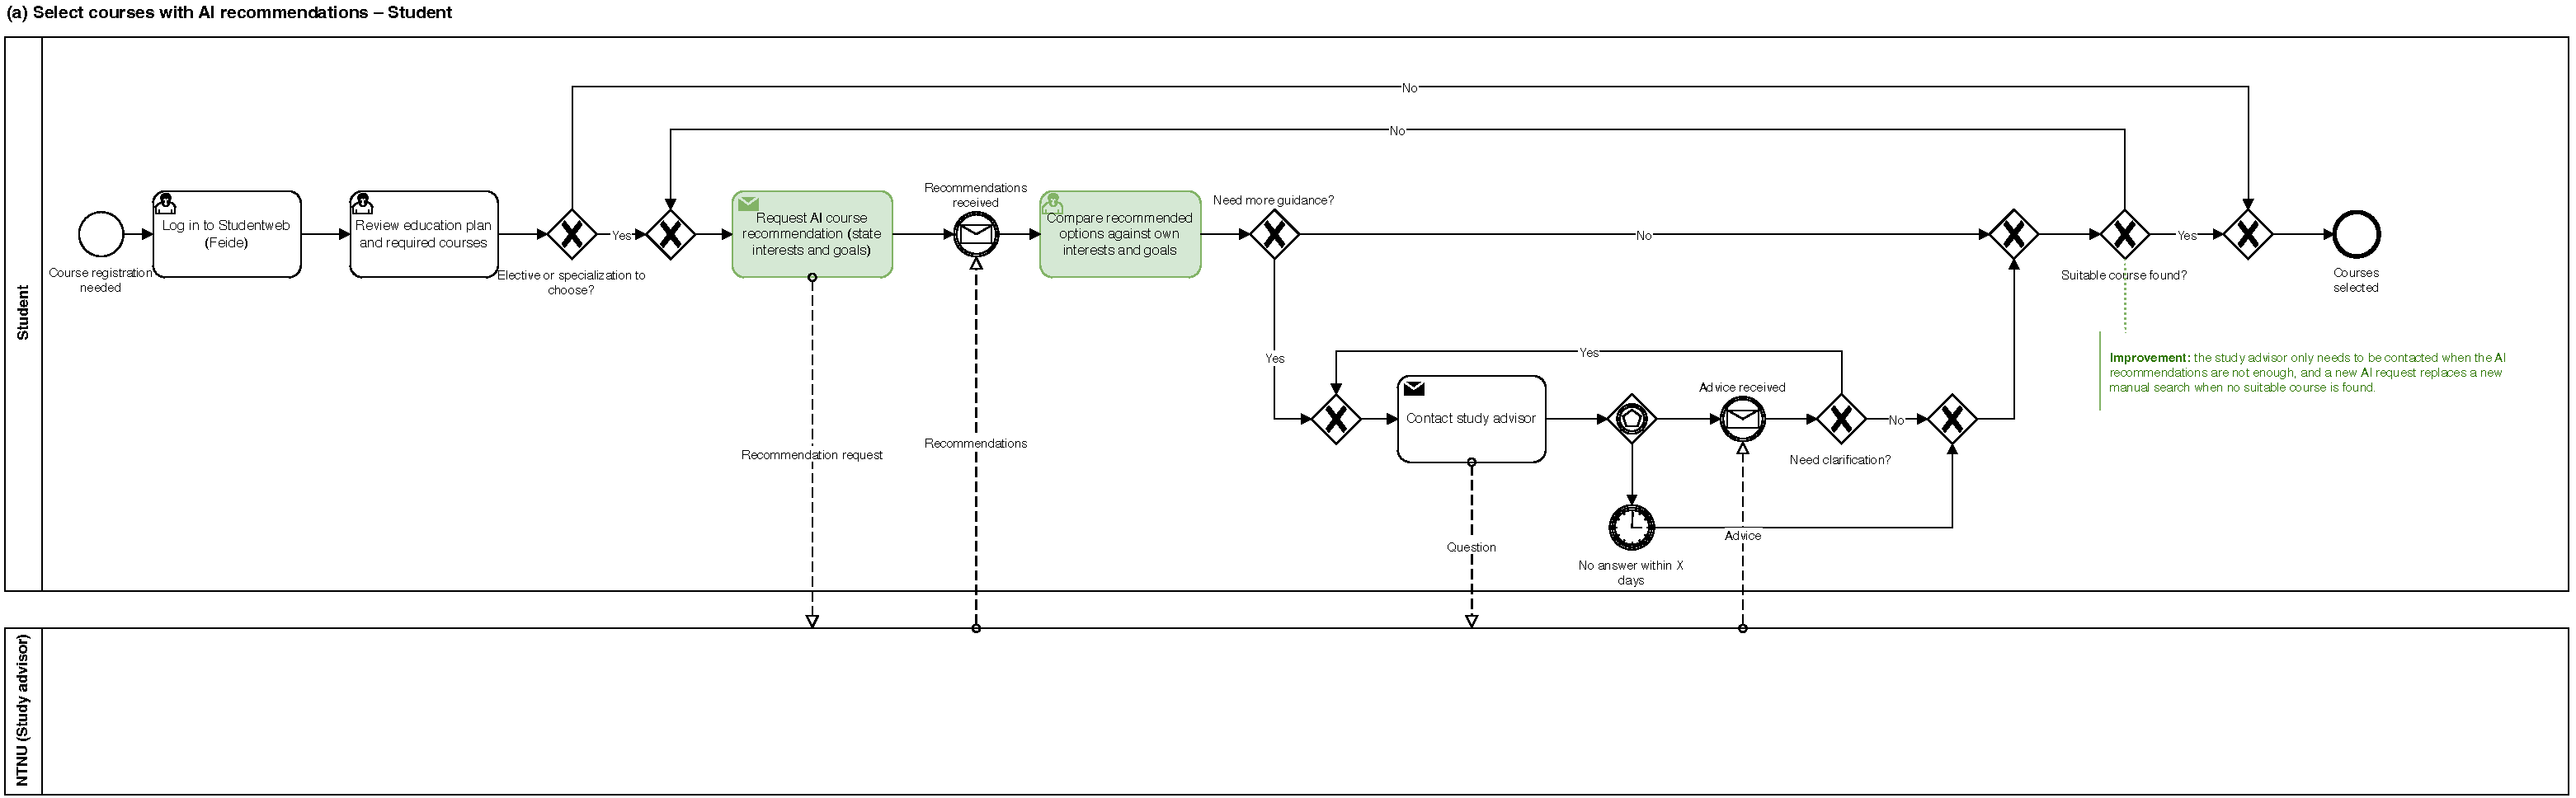
\includegraphics[width=\textwidth]{Images/case3/case3_tobe_a.pdf}
        \caption{Select courses with AI recommendations (Student)}
        \label{fig:case3-tobe-a}
    \end{subfigure}

    \vspace{1em}
    \begin{subfigure}{\textwidth}
        \centering
        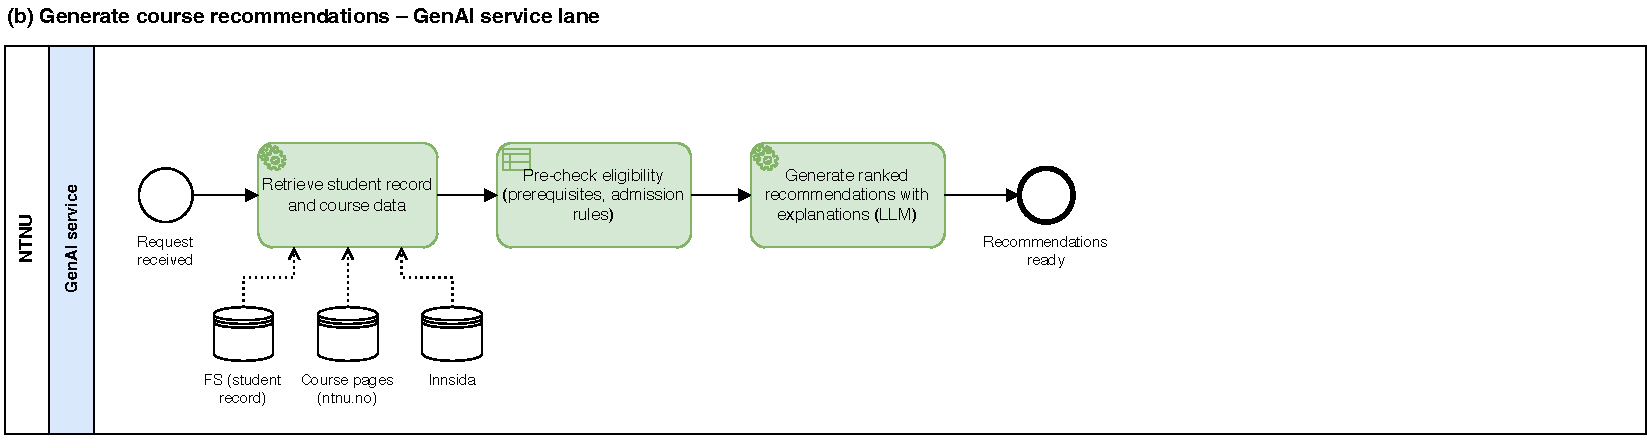
\includegraphics[width=0.75\textwidth]{Images/case3/case3_tobe_b.pdf}
        \caption{Generate course recommendations (GenAI service lane)}
        \label{fig:case3-tobe-b}
    \end{subfigure}

    \vspace{1em}
    \begin{subfigure}{\textwidth}
        \centering
        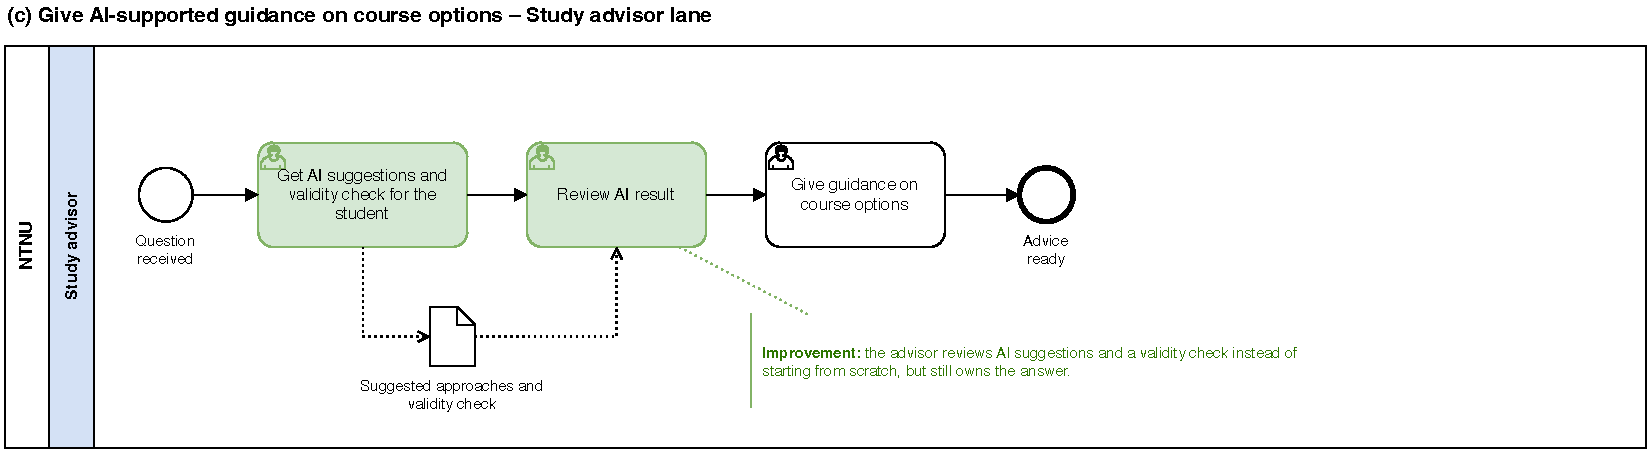
\includegraphics[width=0.75\textwidth]{Images/case3/case3_tobe_c.pdf}
        \caption{Give AI-supported guidance on course options (Study advisor lane)}
        \label{fig:case3-tobe-c}
    \end{subfigure}

    \caption{Case 3 TO-BE BPMN model: expanded sub-processes. Green elements are new or changed compared to the AS-IS model.}
    \label{fig:case3-tobe}
\end{figure}


As described in Section~\ref{sec:case3-asis}, the AS-IS process for course selection has two main pain points. First, students receive no personalized recommendations, and must search for and compare courses manually across several separate sources, such as NTNU course pages and Innsida. Second, guidance depends on the student taking the initiative to contact a study advisor, who must then find an answer manually withput any system support, and the waiting time before an answer is given is unknown. The TO-BE model in Figure~\ref{fig:case3-tobe} addresses these pain points by introducing a GenAI service at two points in the process. Students receive a short list of personalized course recommendations instead of searching on their own (Figures~\ref{fig:case3-tobe-a} and ~\ref{fig:case3-tobe-b}), and study advisors get AI-generated suggestions and an automatic validity check to support their guidance (Figure~\ref{fig:case3-tobe-c}). Since fewer students are expected to need an advisor, and each answer should be faster to produce, the waiting time for guidance may also be reduced, although it is not removed. 

\textbf{Model overview}
Figure~\ref{fig:case3-tobe} shows the TO-BE model for Case 3. In the TO-BE main model (Figure~\ref{fig:main_to-be}), Case 3 is represented by three collapsed subprocesses, each placed in the lane of the actor that performs it. Figure 7 expands all three: (a) Select courses with AI recommendations in the Student pool, (b) Generate course recommendations in the new GenAI service lane, and (c) Give AI-supported guidance on course options in the Study advisor lane. The subprocesses communicate through message flows; the student sends a recommendation request to the GenAI service and receives the recommendations in return, and may send a question to the study advisor and receive advice in return. Activities that are new or changed compared to the AS-IS model are marked green. Subprocess (a) otherwise keeps the same structure as the AS-IS model in Figure 4, so that the differences between the two are easy to see. The registration of courses in Studentweb, where the registration is valid against prerequisites and stored in FS, is unchanged and is shown in the main model. 

\textbf{Subprocess (a): Select courses with AI recommendations}
The first part of the student's process is unchanged from the AS-IS model. The student logs in to Studentweb, reviews their education plan and required courses, and checks whether there are elective or specialization courses to choose. If not, the subprocesses ends directly. If there are, the student no longer researches course options manually. Instead, the student sends a request to GenAI service, stating their interests and goals, and the process waits until the recommendations are received. How the recommendations are generated is described under subprocess (b). The student then compares the recommended courses against their own interests and goals. This task existed in the AS-IS model as well, but it now starts from a short, personalized list instead of every available course across the NTNU course pages and Innsida. This addresses the first pain point, as the student no longer has to search and compare across several separate courses. After comparing the options, the student decides whether more guidance is needed. If so, the student contacts a study advisor, and the student side of this interaction is the as in the AS-IS model; an event-based gateway waits either for the advice to arrive or for a given number of days to pass, and the student can ask for clarification if needed. Finally, the student decides whether a suitable course has been found. If not, the student sends a new request to GenAI service, for example with adjusted interests or goals, instead of starting a new manual search. If a suitable course has been found, the subprocess ends with Courses selected, and the student continues to registration in the main model.

\textbf{Subprocess (b): Generate course recommendations}
Subprocess (b) represents the new GenAI course recommender, placed in its own lane in the NTNU pool. It is started when a recommendation request from a student is received, and consists of three automated tasks. First, the service retrieves the student's record from FS, NTNU's student database, together with course data from the NTNU course pages and Innsida. The student record contains the student's study program, completed courses and grades, and the course data describes the content, prerequisites and admission rules of each course. Second, the service checks which courses the student is eligible for, by comparing the prerequisites and admission rules of each course against the student record. This is modeled as a business rule task, since eligibility is decided by fixed rules and not by the language model. Third, the large language model (LLM) ranks the eligible courses according to the interests and goals stated by the student, and writes a short explanation of why each course fits the student's profile. The result is a ranked short list of courses with explanations, which is sent back to the student. 

The order of these tasks is deliberate design choice. Since the eligibility check is done before LLM, the LLM only ranks and explains courses the student can actually take. This reduces the impact of a known weakness of GenAI, namely that it can produce output that sounds convincing but is incorrect (Qian 2025). It also means that fewer registrations are expected to be rejected, although every registration is still validated in Studentweb as in the AS-IS process. In terms of the types of information systems described by Stair and Reynolds (2018), the recommender can be seen as a decision support system, meaning it supports the student's choice of courses, but the final decision is still made by the student. 

\textbf{Subprocess (c): Give AI-supported guidance on course options}
Subprocess (c) is performed by the study advisor and starts when a question from a student is received. In the AS-IS model, the advisor answered the question without  any system support, by looking up the student's record and searching the course page manually. In the TO-BE model, the advisor first uses the GenAI service to get suggestions for the student. The service returns suggested solution approaches, such as alternative courses or ways to structure the remaining study plan, together with an automatic validity check that confirms whether the courses in question meet their prerequisites and admission rules for this particular student. This is the same eligibility check as in subprocess (b). The result is shown in the model as the data object "Suggested approaches and validity check". The advisor then reviews the AI result and decides what to use from it, before giving guidance to the student as in the AS-IS model. The AI therefore acts as a sparring partner for the advisor rather than replacing the advisor. Keeping a human in the loop is important, since output from GenAI can be incorrect and needs to be checked (Qian 2025). The advisor remains responsible for the answer the student receives. When the advice is ready, it is sent back to the student, who receives it in subprocess (a). This addresses the second pain point, as the guidance is now supported by a system and should be faster to produce. However, the student must still take initiative to contact the advisor, and the waiting time is reduced but not removed. 

\textbf{SusAF analysis}
to be continued



